%\part{付録}
%\parttoc
\appendix

%%%%%%%%%%%%%%%%%%%%%%%%%%%%%%%%%%%%%%%%%%%%%%
\chapter{導出原理}
\label{sec:resolution-principle}

本章では導出原理について概説する.

定理証明において仮定 $A$ から $B$ が結論できること
すなわち $A\vdash B$ を示すためには,$A$ を仮定して
あれこれ推論規則を適用することによって $B$ を導く.
導出原理による証明の場合は,次の同値関係
\[
\begin{array}{l c l c l}
 A \vdash B & \iff & \{A, \neg B\} \vdash \makebox{□ (矛盾)}
 & \iff & \{A, \neg B\} \makebox{が充足不能}
\end{array}
\]
を用いて $\{A, \neg B\}$ が充足不能であることを示すことによって
間接的に $A\vdash B$ を証明する\footnote{ここで $\iff$ は if and only
 if の意味.}.

以下このことを順を追って見てゆくことにする.

\section{節形式と節集合}
閉じた式(閉式---変数を含まない場合も含めて全ての変数が束縛されている論
理式)$A$が妥当であることと $\neg A$ が充足不能であることは同じ事である.
つまり $\neg A$ が充足不能であることを示すことが出来れば $A$ が妥当で
あると結論付ける事ができる.
そこで式の充足不能性を確かめることを考察する.

この時スコーレム標準形(Skolem normal form)と呼ばれる,冠頭標準形に
全称限量子しか含まれない論理式の形式である.任意の一階述語論理式は
充足可能性を保存するスコーレム標準形に変換できる.この変換を
スコーレム化(Skolemization)と呼ぶ.スコーレム化によって得られる式は
元の式が充足されるときそのときに限って充足される.

\section{導出}
導出(resolution)は2つの節を前提として新しい節(導出節)を
導く推論規則である.簡単のためまず命題論理の世界に範囲を
限定する.たとえば $A_1, A_2, A_3$ を命題として
$\neg A_1\lor A_2, \neg A_2\lor A_3$ から
$\neg A_1\lor A_3$ を導くのが命題論理での導出の例である.


%%%%%%%%%%%%%%%%%%%%%%%%%%%%%%%%%%%%%%%%%%%%%%
\chapter{反駁エンジンの動作の詳細}
\label{sec:process-in-detail}

本章では反駁エンジンの推論過程についてより詳細な説明を行う.

\section{推論ループの構造}
反駁エンジンは, 推論終了あるいは中断の条件が検知されるまで, 
指定された推論ルールにしたがって導出節を生成しつづける. 
この処理の構造は以下の通りである.

\begin{enumerate}
\item 現在の主ループ状態を「処理継続」に設定する.

\item 推論ループのための初期化処理を実行する.
  (第 ~\ref{sec:system-init} 節).

\item 初期化処理の結果, システム状態が「処理継続」ならば
  sos から1つ節を選択しこれを given-clause とする.

\item given-clause が存在し, かつシステム内部状態が「処理継続」
  である限り, 以下の処理を繰り返す.
  \begin{enumerate}
  \item 統計情報 cl-given に 1 を加える.
  \item フラグ print-given が on の場合, given-clause を印字する
  \item given-clause を usable の最後に追加する.
  \item given-clause からフラグで指定されている推論ルールを用いて, 節を
    導出する. 
    (第~\ref{sec:infer} 節, 第~\ref{sec:post-process}) . 
  \item 現在のシステム状態が終了条件に合致する物かどうかを調べる.
    (第~\ref{sec:ending-process})
  \item システムの現在状態が「処理継続」以外ならば
    終了状態に関するメッセージを
    出力し, ループを抜け出す.
  \end{enumerate}
\end{enumerate}

以降で初期化から始まり,節の導出,導出後の処理,終了判定の各
プロセスについて詳細に説明する.

\section{システムの初期化}
\label{sec:system-init}

\texttt{resolve} コマンドが発せられると反駁エンジンが起動される.
その際反駁エンジンは主ループに入る前に
実行文脈の設定に続いて推論処理のための初期化処理を行う.

まず最初に反駁エンジンの実行文脈とするCafeOBJモジュールに関しての
推論の準備を行う.
\begin{enumerate}
\item オペレータの優先順位を設定する.
\item モジュールの公理を節形式へ変換する.
\end{enumerate}

次いで反駁エンジンの主ループに入る前に, 以下のような初期化処理が
実行される.

\begin{enumerate}
\item フラグ universal-symmetry が on の場合に, 
  対称則(X = X)を入力節に追加する.
\item 統計情報を全て 0 に初期化する.
\item フラグ auto あるいは auto2 が on の場合にそれに応じたフラグや
  パラメータの自動セッティングを行う.
\item 実行文脈のCafeOBJモジュールに含まれる built-in demodulator を登
  録する. 
\item フラグ process-input が on の場合, sos および usable 
  に含まれる各節に対して導出節の事前/事後処理(第 ~\ref{sec:pre-process}
  節および第 ~\ref{sec:post-process} 節を参照) を適用する.
\end{enumerate}

\section{導出節生成エンジン群の起動}
\label{sec:infer}

システムの初期化処理に続いて
フラグで指定されている推論規則に対応した
導出節生成エンジン群が順次起動され, 新たな導出節が生成され,
sos に追加される.

\begin{enumerate}
\item max-weight パラメータの調整(\ref{sec:pn-control-memory}節)
  \begin{enumerate}
  \item もしフラグ control-memory が on であれば, 現在の sos 節集合に
    登録されている節の数を調べ, 必要ならば max-weight パラメータを調整する.
  \end{enumerate}
\item binary resolution の実行
  \begin{enumerate}
  \item もしフラグ binary-res が on であったならば, 
    binary resolution を実行する
    (第~\ref{sec:binary-res}節を参照). 
  \item binary resolution の結果得られた新たな導出節の各々について
    導出節の後処理を実行する(第 ~\ref{sec:post-process} 節を参照 --- 以下同様). 
  \end{enumerate}

\item hyper resolution の実行
  \begin{enumerate}
  \item もしフラグ hyper-res が on であったならば, 
    hyper resolution を実行する(第~\ref{sec:hyper-res}節を参照).
  \item hyper resolution の結果得られた新たな導出節の各々について
    導出節の後処理を実行する. 
  \end{enumerate}

\item negative hyper resolution の実行
  \begin{enumerate}
  \item もし, フラグ neg-hyper-res が on であったならば, 
    nagtive hyper resolution を実行する (第~\ref{sec:neg-hyper-res} 節
    を参照). 
  \item negative hyper resolution の結果得られた新たな導出節の各々について
    導出節の後処理を実行する. 
  \end{enumerate}

\item paramodulation into の実行
  \begin{enumerate}
  \item もし, フラグ para-into が on であったならば, 
    paramodulation (into) を実行する
    (第~\ref{sec:paramod}節を参照).
  \item paramodulation (into) で得られた新たな導出節の各々について
    導出節の後処理を実行する. 
  \end{enumerate}

\item paramodulation from の実行
  \begin{enumerate}
  \item もし, フラグ para-from が on であったならば, 
    paramodulation (from) を実行する
    (第 ~\ref{sec:paramod} 節を参照).
  \item paramodulation(from) で得られた新たな導出節の各々について
    導出節の後処理を実行する.
  \end{enumerate}
\end{enumerate}  

\subsection{max-weight パラメータの調整}
\label{sec:pn-control-memory}

推論実行中の sos の爆発を避けるために用意されているパラメータが
max-weight である. このパラメータ値を越えるサイズを持つ導出節は
sos に登録されずに捨てられる. 

さらにそのサイズが一定の目安を越えた場合に, max-weight 
パラメータの値を自動調整することも行う. 
これはフラグ control-memory が on になっている場合に実行される.

\subsection{節に対する前処理}
\label{sec:pre-process}

各入力節(フラグ process-input が on の場合)や
導出された節に関して, 
例えば max-weight パラメータで制限される節の重さ等, 
さまざまな制約条件や論理的に冗長な節であるかどうかの検査(subsumption
や tautology)を実行し, 残すべき節か捨てる物かを判別する.
また dymanic demodulator の生成や空節が生成されたか否かの検査等を実行する.
具体的な処理の内容は以下の通りである:

\begin{enumerate}
\item 節を調べ結果として残すべきか否かを調べる
  (第~\ref{sec:proc-gen} 節を参照).
  結果が捨てるべき節となった場合は
  その節を削除する.
\item 節の重みを計算する.
\item 統計情報 cl-kept の値に 1 を加える
\item フラグ print-kept が on であるか, 入力節に対する処理であった場合
  clause を印字する.
\item フラグ dynamic-demod が on であり, dynamic demodulator に関する検査
  (第~\ref{sec:dynamic-demodulator} 節)の結果が demodulator として
  ふさわしい節と判定された場合, それから新たな demodulator を作成する.
  この時フラグ print-new-demod が on であるかあるいは入力節に対する
  処理であった場合, 作成した demodulator を印字する.
\item 空節の検査を行う.
  空節であった場合,
  \begin{enumerate}
  \item もしパラメータ max-proofs が -1 (得られる証明の数に制限を設け
    ない)ではなく,
    導出された空節の数(統計情報 empty-clauses) の値が, パラメータ
    max-proofs に達していたら, システム状態を「最大証明数に達した」
    として反駁エンジンを中断する(大域的脱出). 
  \end{enumerate}
\end{enumerate}

\subsection{節に対する処理の検査内容}
\label{sec:proc-gen}

\begin{enumerate}
\item 節の変数名を付け替え,これを clause とする
\item フラグ very-verbose が on であれば clause を印字する
\item clause に demodulation を施す.

  もしフラグ very-verbose が on 
  であり, 書き換えが一度でも実行されていれば書き換え結果の clause を
  印字する.

\item 等式の左右辺の方向つけ

  フラグ order-eq が on の場合に実行する.
  このとき
  \begin{itemize}
  \item フラグ lrpo が on であれば, lrpo(lexicographic recursive path ordering)
    による順序つけを用いる(第~\ref{sec:orient-lrpo} 節を参照).
  \item そうでなければ, 辞書式順による等式の順序つけを行う
    (第~\ref{sec:orient} 節を参照)
  \end{itemize}
\item unit deletion 処理を施す.

  フラグ unit-deletion が on であり,かつ
  clause に含まれるリテラルの数が 2 以上の
  場合に実行する(第 ~\ref{sec:unit-deletion} 節を参照).
    
\item  factor simplification の実行

  フラグ factor が on の場合に実行する
  (第 ~\ref{sec:factor-simplify} 節を参照).
  この時 simplification を行った回数分
  統計情報 factor-simplifications を増やす.

\item tautology の検査

  節が tautology か否かを調べる(第 ~\ref{sec:cl-tautology?} 節
  を参照). もしそうならば統計情報 cl-tautology を 1 増やす.
  このような節は推論に寄与しないためこの節を「残すべきでない」と判定する.

\item weight のテスト(導出節に対してのみ行い, 入力節に対しては
  実施されない):
    
  節の重さがパラメータ max-weight を
  越えいた場合, この節を「残すべきでない」と判定する.
  この時フラグ very-verbose が on であったならば, その旨印字する.

\item forward subsumption テスト

  フラグ for-sub が on の場合に実行する(第 ~\ref{sec:forward-subsume}
  節を参照).
  
  結果として検査している節が他の節に subsume されるような節であった場合は,
  この節は冗長のため「残すべきでない」と判定し,
  統計情報の cl-for-sub に 1 を加える. また, clause を subsume する節が
  sos 節集合に含まれているものであった場合は, 統計情報 cl-for-sub-sos に
  1 を加える. さらにフラグ very-verbose が on であるか, 入力節に対する
  処理であった場合は, 節が subsume された旨を印字する.
  
\end{enumerate}


\subsection{Unit Deletion}
\label{sec:unit-deletion}

これは導出に使用する節を簡素化することが目的であり,
節に含まれるリテラルの数が 2 以上の場合に行われる.
この処理の対象とする各リテラル $l_i$ について, sos あるいは usable に
含まれる単一節のリテラルのうち, インスタンスが $l_i$ の否定に等しくな
るものが存在する場合に, リテラル $l_i$ を削除する処理である.

\subsection{Tautology 検査}
\label{sec:cl-tautology?}

\begin{verbatim}
     P | ... | ~P | ...
\end{verbatim}
という形をした節は tautology であるので, 以降の推論の役には立たない. 
このような節であるかどうかを判定するのが Tautology 検査である.

\subsection{Subsumption テスト}
\label{sec:subsume?}

節 $C$ が 節 $D$ を subsume するとは, 
$D$ に含まれる全てのリテラルが $C$ のどれかのリテラルを
インスタンス化する事によって得られるような場合である.
つまり $C$ の方が $D$ より一般的な節であるという事ができる.
このような場合節 $D$ は冗長であり, $C$ があれば新たな導出節の生成に寄
与しない.
この検査を行うのが Subsumption テストである.

\subsection{Forward Subsumption テスト}
\label{sec:forward-subsume}

導出された節が sos あるいは usable に含まれる節によって subsume される
場合, この節は以降の推論には役に立たない(冗長である). 
この検査を forward subsumption テストと呼ぶ.

\section{節に対する後処理}
\label{sec:post-process}
節に対する後処理とは, 前処理(第~\ref{sec:pre-process}節)を通った
節に関して行われる処理である. 
この処理にある節が渡される時点では, すでにその節は適切な節集合
(sos あるいは usable)に追加されいる.

前処理では節の有効性を判定する検査が既存の切に照らし合わせて種々行われ
ていたのに対して,
後処理では逆に新たな導出節によって冗長になるような既存の節が
あるかどうかを調べる.
そのような節が存在した場合は,状況に応じて削除(back subsumption)したり,
新たに生成された demodulator によって既存の節を簡約化(back demodulation)
したりする. また factoring によってさらに新たな節が生成されることもある.

具体的には以下のような処理が実行される:

\begin{enumerate}
\item 等式の入れ換え

  フラグ eq-units-both-ways が on かつ, 処理対象の節が単一節であり
  そのリテラルが equality リテラル(等式のリテラル)の場合に
  以下の処理を行う:
  \begin{itemize}
  \item フラグ order-eq が off であるか, あるいはリテラルの
    等式を向きつけることが出来なかったものであったならば, 以下の処理を
    行う. そうでなければなにもしない.
    \begin{enumerate}
    \item 等式の左右辺を入れ換えたリテラルを作成し,
    \item これを唯一のリテラルとする新たな単一節を作成する
    \item 作成した節の導出履歴に copy-rule と flip-eq-rule を追加する
    \item 作成した節を, 導出節前処理 -- 第 ~\ref{sec:pre-process}節 -- 
      にかける. 
    \end{enumerate}
  \end{itemize}

\item back demodulation の実行

  フラグ back-demod が on かつ, clause に対応する demodulator
  が前処理で生成されていた場合に実行する.
  back demodulation は \ref{sec:back-demodulate} 節を参照.

\item back subsumption のテスト

  フラグ back-sub が on の場合に行う(第 ~\ref{sec:back-subsume} 節を参照).
  clause に subsume された節の数の分だけ統計情報 cl-back-sub を増やす.
  このとき print-back-sub フラグが on であるか, 入力節に対する処理で
  ある場合には, back subsume した旨メッセージを印字する.

\item factoring

  フラグ factor が on の場合に行う.
    
\item back unit deletion 
    
  フラグ back-unit-deletion が on かつ clause が単一節の場合に行う.
  第 ~\ref{sec:back-unit-deletion} 節を参照.
\end{enumerate}


\subsection{Back Subsumption テスト}
\label{sec:back-subsume}

導出された新たな節が, sos あるいは usable に含まれている節を subsume 
するような場合, subsume される節は冗長であるから削除することが出来る.
この検査を back subsumption テストと呼ぶ.

\subsection{Back Unit Deletion}
\label{sec:back-unit-deletion}

導出節が単一節の場合, そのリテラルと符号が逆で照合可能なリテラル
を削除することによって節を簡単化することが出来る. 
これを sos および usable に含まれる全ての節に対して実行するのが
back unit deletion である.

\section{推論終了の判定}
\label{sec:ending-process}

推論途中ではパラメータの値や空節の導出を監視して推論の中断/終了の判定を
行う. 
まずパラメータによる
終了条件の判定は以下のように実行され, それに伴ってシステム内部状態が設
定される.
\begin{enumerate}
\item パラメータ max-given が -1 ではなく, 統計情報の cl-given が
  max-given 以上の場合, 状態を「max-given で終了」とする.
\item パラメータ max-gen が -1 ではなく, 統計情報の cl-generated が
  max-gen 以上の場合, 状態を「max-gen で終了」とする.
\item パラメータ max-kept が -1 ではなく, 統計情報の cl-kept が
  max-kept 以上の場合, 状態を「max-kept で終了」とする.
\item 上記以外なら「処理継続」とする.
\end{enumerate}

空節の判定は次のようにして行う.
\begin{enumerate}
\item 節に含まれるリテラルの数が 0 の場合.

  これは空節であり, 以下の処理を実行する.
  \begin{enumerate}
  \item フラグ print-message が on であれば空節が導出された旨印字する.
  \item 統計情報 cl-kept を 1 増やす.
  \item 節が含まれている節集合からこの節を削除する.
  \item 統計情報 empty-clauses を 1 増やす.
  \item フラグ print-proofs が on であれば証明木を印字する.
  \end{enumerate}

\item リテラルの数が一つの場合(単一節)

  unit conflict があるかどうかを調べる(第 ~\ref{sec:unit-conflict} 節を参照).
  その結果 unit conflict となった場合, 以下の処理を行う. 
  \begin{enumerate}
  \item print-message フラグが on の場合 unit confict となった旨印字する.
  \item フラグ print-proofs が on の場合証明木を印字する.
  \item 節の含まれている節集合からこの節を削除する.
  \end{enumerate}
\end{enumerate}

\subsection{Unit Conflict 検査}
\label{sec:unit-conflict}

与えられた単一節を反駁するような, sos あるいは usable に
含まれる単一節の全てを探し, もしあればそれぞれについて反駁を
実行して空節を作り出す処理である.

\subsection{Factoring 処理}
\label{sec:factoring-proc}

節 $C$ に含まれる 2つ以上の(同じ符号の)リテラルに,mgu(most general unifier)
$\sigma$ があるとしたとき,$\sigma C$ ($C$ の各リテラルのアトムに, $\sigma$ 
を適用した結果) を $C$ の factor と呼ぶ.

例えば,
$C = \underline{P(x)}\lor \underline{P(f(y))} \lor 〜Q(x)$ としたとき,
(下線を引いた)最初と2番目のリテラルは,mgu $\sigma = \{f(y)/x \}$ を持つ.
したがって,$\sigma C = P(f(y))\lor 〜Q(f(y))$ は $C$ の factor である.

\subsubsection{Factor Simplification 処理}
\label{sec:factor-simplify}

factor simplification は, ある節の factor が元の節を subsume する
ものかどうかを調べ, そうであれば元の節のリテラルを factor の
リテラルで置き換える. このようにして clause を簡単化して, 冗長な
リテラルを削除して行く処理である.

%%%%%%%%%%%%%%%%%%%%%%%%%%%%%%%%%%%%%%%%%%%%%%%%%%%%%%%%%%%%%%%%%%%%%%
\chapter{推論ルール概説}
\label{sec:desc-resolution}
本章では各種の節導出方式について簡単に説明する.

\section{Binary Resolution}
\label{sec:binary-res}

binary resolution はリテラルとリテラル 1 対 1 の通常の resolution ルールである.
resolution のスキームは図 \ref{fig:binary-res} に示す通りである:
\begin{figure}[htbp]
  \begin{center}
    $$
    \infer{
      \begin{array}{ll}
        \mbox{\textbf{binary resolvent:}} &
        \sigma K_1, \cdots, \sigma K_k, \sigma M_1,\cdots,\sigma M_m
      \end{array}
      }
    {\begin{array}{ll}
        \mbox{\textbf{clause-1:}}& 〜L', M_1,\cdots,M_m \\
        \mbox{\textbf{clause-2:}}& L,K_1,\cdots,K_k
      \end{array}\;\;\;\;\sigma は L と L' の mgu
      }
    $$
    \caption{{binary resolution のスキーム}}
    \label{fig:binary-res}
  \end{center}
\end{figure}

図に示したスキームで, 二つの親節は同一の変数項を共通して持っていてはならない.
この条件は, 生成節の変数は常にユニークになるように変数のつけ替えが行われて
いるため, 自動的に満足されている. 

%%%
\section{Hyper Resolution}
\label{sec:hyper-res}
\label{sec:neg-hyper-res}

ある節から導かれる導出節を考えた場合, それを得るのに
異なった導出ステップがあり得る. 
従って, 同じ導出節が複数回生成される場合があり得る.
これは望ましくないので, この複数のステップをまとめて
一度の resolution によって導出しようとするのが hyper resolution
である.

反駁エンジンでは,positive hyper resolution と negative hyper resolution
の2種の hyper resolution 機能を提供しているが,これらはいずれも
一種の semantic resolution であり,PI-resolution と呼ばれるより一般的な
resolution rule の特殊形である.

ここではまず最初に,この semantic resolution の考えかたについて説明し(\cite{chang-lee}),
ついで,hyper resolution のスキームについて説明する.

\subsection{Semantic Resolution の考え方}\cite{chang-lee}

節の集合 $S$ を,
$S = \{〜P \lor 〜Q \lor R, P\lor R, Q\lor R, 〜R\}$
とする.この節集合の充足不能性を示すのに,通常の binary-resolution を
使うと,以下に示すような演繹過程となる:

\begin{center}
{\small
\begin{tabular}{lll}
(1) & $〜P \lor 〜Q \lor R$ & $S$ の要素 \\
(2) & $P\lor R$ & $S$ の要素 \\
(3) & $Q\lor R$ & $S$ の要素 \\
(4) & $〜R$  & $S$ の要素 \\
(5) & $〜Q\lor R$ & (1) と (2)から\\
(6) & $〜P\lor R$ & (1) と (3)から \\
(7) & $〜P\lor 〜Q$ & (1) と (4) から\\
(8) & $P$ & (2) と (4) から \\
(9) & $Q$ & (3) と (4) から \\
(10) & $〜Q\lor R$ & (1) と (8)から \\
(11) & $〜P\lor R$ & (1) と (9)から \\
(12) & $R$ & (2) と (6) から \\
(13) & $〜Q$ & (4) と (5) から \\
(14) & $〜P$ & (4) と (6) から \\
(15) & □ & (4) と (12) から \\
\end{tabular}
}
\end{center}
導出節のうち,実際に証明に使われているのは (6) と (12) だけである.
その他の導出節は全て冗長である.この様な冗長な節の導出を避けるのが
目的となる.

節を適当な2つのグループ $S_1$ と $S_2$ に分けることが出来たとする.
また, おなじグループに含まれる節同士の間では resolution を行わないとする.
このようにする事で, 導出される節の数が減ることはあきらかである.

semantic resolution では, 節のグループ分けに\textbf{解釈}(interpretation)
を用いる. 上の例で, (2) と (3) は, 解釈 $I = \{〜P, 〜Q, 〜R\}$ では
false である. 一方 (1) と (4) は満足される. このようにすることで, 
$S$ を解釈で true になるものとそうでないものとに分類することが出来る.
反駁エンジンは, 節の充足不可能な節集合を扱うものであるから,
どのような解釈を採用したとしても, それが全ての節を満足したり否定する
ようなことは無い. したがって, どのような解釈によっても節集合を
2つの集合に分類することが可能である.
以下では, 先の例の節集合 $S$ が上で述べた解釈 $I$ によって,
二つのグループ 
$S_1 = \{(2), (3)\}$, $S_2 = \{(1), (4)\}$ に分類されているものとする.
このように分類しても, (2) と (3) は (4) と resolve することが出来る.
以下で述べるように, この resolution についても避けることが可能である.

上のような resolution を回避するため, 述語記号の間の順序付けを使うことが
出来る.
たとえば, $S$ に含まれる述語記号に
\[ P > Q > R \]
という順序を付けるものと仮定する.
この順序付けのもとで, 2つの節(片方は $S_1$ の節, もう片方は $S_2$ の節)
を resolve する場合, resolve されるリテラルで $S_1$ に属する節のものは
最大の述語記号をもっていなければならない, という制約条件を付ける.
この制約のもとでは, $R$ は (2) および (3) で最大の述語記号ではないため,
(2) を (4) と resolve することは出来ないし,また, (3) と (4) に関しても同様である.  

次に semantic resolution で重要となる概念である clash について説明する.
まず, 先の例の節について見てみる.
\begin{enumerate}
\item[(1)] $〜P\lor 〜Q \lor R$
\item[(2)] $P\lor R$
\item[(3)] $Q\lor R$
\item[(4)] $〜R$
\end{enumerate}
解釈 $I$ を $I = \{〜P,〜Q,〜R\}$ とし, 述語記号の順序を 
$P > Q > R$ とする. 上で議論した2つの制約を適用すると, 次の2つの
節のみが導出出来る:
\begin{enumerate}
\item[(5)] $〜Q\lor R$ \hskip4cm (1)と(2)から
\item[(6)] $〜P\lor R$ \hskip4cm (1)と(3)から
\end{enumerate}
これらの両方とも $I$ によって満足される. したがってこれらを $S_2$ へ入れ,
それらを $S_1$ に含まれる節と resolve する. 
(5) は (3) と (6) は (2) と resolve 出来る. 両方とも同じ結果 $R$ になる.
\begin{enumerate}
\item[(7)] $R$ \hskip5cm (3)と(5)から
\item[(8)] $R$ \hskip5cm (2)と(6)から
\end{enumerate}
節 $R$ は $I$ では false なので, それを $S_1$ へ入れ, これと $S_2$ に含まれる
節との間で resolve を行う. $〜R$ が $S_2$ にあるので, 空節 □ を得る.

上の二つの $R$ の導出過程を見ると, ともに節 (1), (2) と (3) が使われている.
異なるのはそれらが使われる順序である. どちらか一つだけが必要であり, 片方は
冗長であり, 極めて無駄である. この冗長性を無くすために, clash という概念を
導入する. clash の考え方は, (1), (2), (3) の3つの節から, 
中間的な節 (5) や (6) を経由せずに, 直接的に $R$ を導出するというものである. 
この例では, 集合 $\{(1), (2), (3)\}$ を clash と呼ぶ. clash の詳細に
ついては, 次のパラグラフで説明する. 

\subsection{PI-resolution の定義}
$I$ を解釈とし,$P$ を述語記号の順序付けとする.
節の有限集合 $\{E_1,\ldots, E_q, N\}$, $q \ge 1$ は
次の条件を満足する時,\textsl{semantic clash} と呼ばれる:
\begin{enumerate}
\item $E_1,\ldots, E_n$ は $I$ で false
\item $R_1 = N$ とする. 各 $i = 1, \ldots q$ について, 
  $R_i$ と $E_i$ の resolvent $R_{i+1}$ が存在する.
\item resolve される $E_i$ のリテラルは, $E_i, i = 1,\ldots q$ の
  うちで最も大きな述語記号を持っている.
\item $R_{q+1}$ は $I$ において false
\end{enumerate}
$R_{q+1}$ を (PI-clash $\{E_1,\ldots,E_q,N\}$ の) PI-resolvent と呼ぶ.
また, $E_1,\ldots,E_n$ を \textbf{electrons}, $N$ を \textbf{nucleus}
と呼ぶ. 

例えば, 
$$
E_1 = A_1 \lor A_3, \hskip1cm E_2 = A_2 \lor A_3, \hskip1cm 
N = 〜A_1 \lor 〜A_2 \lor A_3
$$
とする. 解釈 $I$ を $I = \{〜A_1, 〜A_2, 〜A_3\}$ とし, 順序 $P$ を
$A_1 > A_2 > A_3$ とする. 
この場合, $\{E_1,E_2,N\}$ は PI-clash である. この clash の PI-resolvent 
は, $A_3$ である($A_3$ は $I$ で false であることに注意). 

\subsection{Negative Hyper Resolution}
negative hyper resolution は,上で述べた PI-resolution で
解釈 $I$ に否定記号が含まれていない場合である.

negative hyper resolution のスキームを図\ref{fig:hyper-res}に示す.
\begin{figure}[htbp]
  \begin{center}
    %\epsfxsize=\textwidth
    %\centering\epsfbox{hyper-res.pdf}
    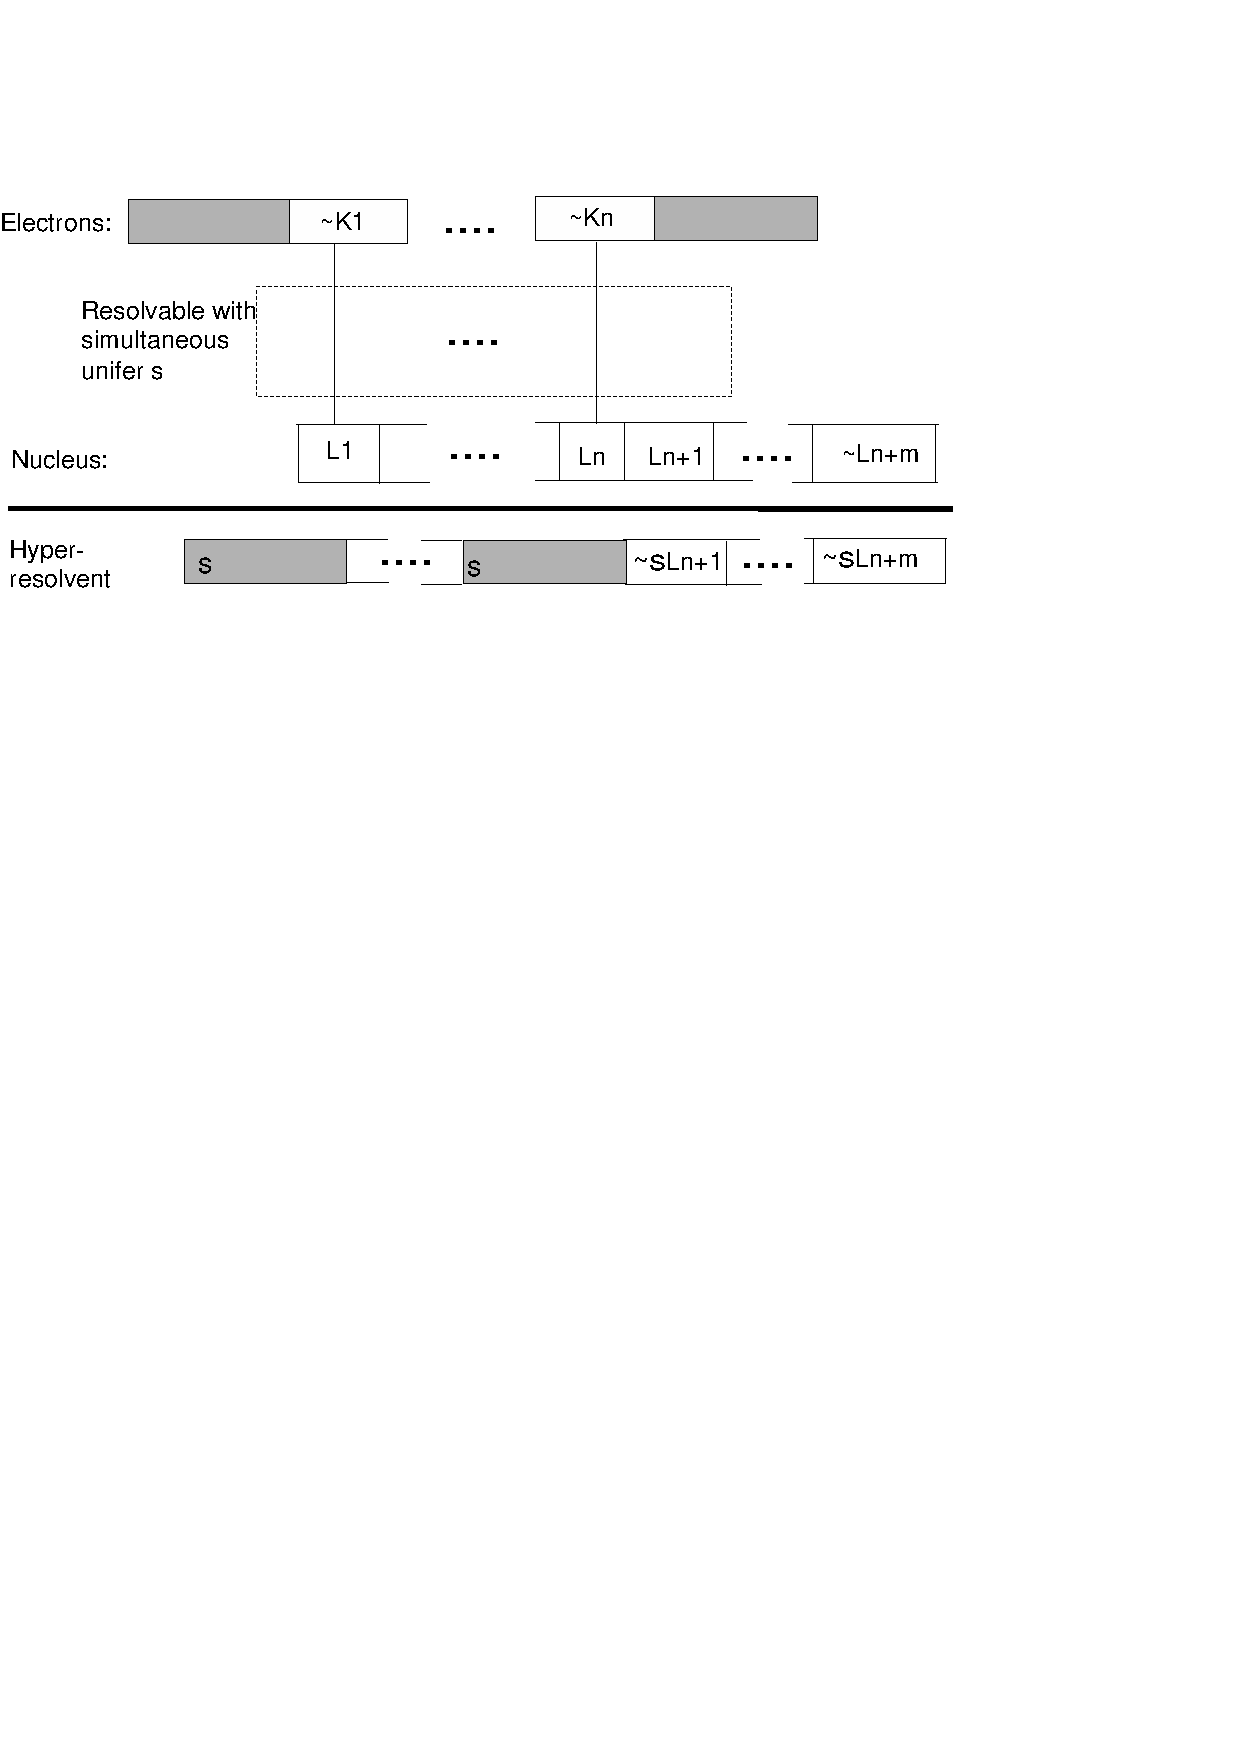
\includegraphics[width=\textwidth]{hyper-res.pdf}
    \caption{{hyper resolution のスキーム}}
    \label{fig:hyper-res}
  \end{center}
\end{figure}

図で nucleus とあるのは, 少なくとも一つの正のリテラルをもつ節である.
反駁可能な節集合にはこのような節が必ず存在する.
nucleus の個々の正のリテラルにつき, 負のリテラルのみを持つ節 electron が必要である.
やはり, 反駁可能な節集合にはこのような節が必ず存在する.
nucleus は全ての electron と「同時に」resolve されなければならない. 
結果として負のリテラルのみからなる節が, 導出節として得られる(図の hyper-resolvent).
この導出節は, 以降の hyper-resolution ステップで electron として使用することが出来る.

我々の反駁エンジンでは, フラグ neg-hyper-res が on の時に
使用される negative-hyper-resolution に相当する.

\subsection{Positive Hyper Resolution}

フラグ hyper-res が on の時に使用されるのは, これと dual な関係にある,
\textsl{positive} hyper resolution である. 
これは, 上で述べたスキームで, リテラルの 正/負 を逆にする事で得られ,
PI-resolution で,解釈 $I$ に含まれる各リテラルが否定記号を含む場合に
相当する.

否定の形で与えられる結論は, 通常負のリテラルのみを含むことが多いため,
negative hyper-resolution の electron として用いる事が出来るので,
結論から仮定へ向かっての, 後向き推論に適していると言える.
一方 positive hyper-resolution は, 仮定から結論へ向けての, 前向きの
推論が可能である. 

%%%%%%%%%%%%%%%%%%%%%%%%%%%%%
\section{Paramodulation}
\label{sec:paramod}

paramodulation は等号を扱うための推論ルールである. 
図~\ref{fig:paramod-rule} に paramodulation のスキームを示す.
図で, $l = r$ は \textbf{paramodulator} (正の等式リテラル), 
$f(t)$ は $t$ を副項に持つようなリテラル
である. $f(\sigma{r})$ は, その $t$ を $\sigma(r)$ で置き換えた項を
表すものとする.

\begin{figure}[htbp]
  \begin{center}
    $$
    \infer{
      \begin{array}{ll}
        \mbox{\textbf{paramodulant:}} &
        f(\sigma r), \sigma L_1,\cdots,\sigma L_n,\sigma M_1,\cdots,\sigma M_m
      \end{array}
      }
    {\begin{array}{l}
        l = r, L_1,\cdots,L_n \\
        f(t), M_1,\cdots,M_m
      \end{array}\hskip2cm\sigma は l と t の mgu
      }
    $$
    \caption{{paramodulation のスキーム}}
    \label{fig:paramod-rule}
  \end{center}
\end{figure}
図で, $sigma$ は, リテラル $f(t)$ の副項 $t$ と paramdulator の
左辺 $l$ との mgu(most general unifier) である ($\sigma l = t$).
paramodulant は $t$ を paramodulator の右辺に $sigma$ を適用した
もの($f(\sigma r)$) で置き換えることによって得られる.

%%%%%%%%%%%%%%%%%%%%%%%%%%%%%%%%%%%%%%%%%%%%%%%
\section{Demodulation}
\label{sec:demod}

demodulation は,導出された節に適用され,それに含まれるリテラルのアトムを
簡約化する.
すなわち,$l\rightarrow r$ の形をした demodulator があり,あるリテラル
$l$ が項 $t$ を副項として含む $P[t]$ の形をしているものとする.
このとき,$\sigma l = t$ となるような,変数置換があったときに,
$l$ を,$P[\sigma r]$ に書き換える.

demodulator として,$L = R$ という等式のリテラルのみからなる節が用いられる.
これを,項の書き換え規則として用いるためには,
等式の方向付けが必要である.
つまり,何らかの順序関係によって,等式の左右辺を方向付ける必要が
ある.反駁エンジンでは,この順序の判定に,単純な辞書式順と lrpo の 2種 を用意する.

\subsection{実行時のdemodulator判定}
\label{sec:dynamic-demodulator}

フラグ dynamic-demod が on の場合, 反駁エンジンは,
全ての equality ($\alpha = \beta$)を demodulator として使えるか
どうかを判定する.

フラグ dynamic-demod あるいは, dynamic-demod-all が on になっている
状況では, 必ずフラグ order-eq が on になっているはずである.
この時フラグ lrpo が on の場合には, 等式の向きつけの判定として
LRPO を,
そうでない場合は単純な重みと辞書式順による比較が行われる.
この結果等式の向きつけが行われるが, その
節が demodulator として使えるかどうかは, 次のような処理で
判定される.
なお検査の対象とする節は, 正の equality かつ単一節である.

\begin{enumerate}
\item 節のリテラル $l (\alpha = beta)$ に関して以下の判定を実行する:
  \begin{description}
  \item[フラグ lrpo が off の場合]
    \begin{enumerate}
    \item $\beta$ が $\alpha$ の副項であれば :normal とする
    \item 辞書式順の意味で 
      $\alpha > \beta$ かつ $vars(\alpha) \supseteq vars(\beta)$
      ならば,
      \begin{enumerate}
      \item フラグ dynamic-demod-all が on であれば OK とする
      \item dynamic-demod-all が off で $wt(\beta)\leq 1$ ならば
        OK とする
      \item それ以外の場合は NG とする
      \end{enumerate}
    \item フラグ dynamic-demod-lex-dep と dynamic-demod-all の
      両方が on のとき, $\alpha$ と $\beta$ が変数を除外すれば,
      構文的に同一の項である場合に ORDER-DEP とする.
    \item それ以外の場合は NG とする
    \end{enumerate}
  \item[フラグ lrpo が on の場合]
    \begin{enumerate}
    \item $l$ の等式の向きつけが正しく行われている場合, OK とする.
    \item フラグ dynamic-demod-lex-op が on の場合,
      $vars(\alpha)\supseteq vars(\beta)$ ORDER-DEP とする.
    \item それ以外の場合は NG とする
    \end{enumerate}
  \end{description}
\end{enumerate}

上の処理で, $vars(t)$ は, 項 $t$ に出現する変数の集合を意味する.

\subsection{Back Demdulation の実行}
\label{sec:back-demodulate}

back demodulation とは,導出された節が正の単一の equality 節
(一つの $\alpha = \beta$ の形のリテラルのみからなる節) で
あった場合に,それを demodulator として用いて,usable および
sos に含まれる全ての節に関して demodulation を実行するものである.

導出節が demodulator として適切なものかどうかの判定は,
導出節に対する前処理(第\ref{sec:pre-process}節
を参照)で行われている.

%%% Local Variables: 
%%% mode: latex
%%% TeX-master: t
%%% End: 
